\documentclass{article}

%--------------------------------------------------------------
% Document & Font Setup
%--------------------------------------------------------------
\usepackage[a4paper, margin=1in]{geometry}
\usepackage{setspace}
\usepackage{parskip}
%--------------------------------------------------------------
% Common Packages
%--------------------------------------------------------------
\usepackage{graphicx}
\usepackage{subcaption}
\usepackage{caption}
% Subfigure captions
\DeclareCaptionLabelFormat{custom}{\figurename~\thefigure~(#2)}
\captionsetup[subfigure]{labelformat=custom}

\usepackage{enumitem}
\usepackage{float}
\usepackage{placeins}
\usepackage[dvipsnames,x11names,svgnames]{xcolor}
\usepackage{url}

%--------------------------------------------------------------
% Math & Science Packages
%--------------------------------------------------------------
\usepackage{amsmath,amssymb,amsfonts,amsthm}
\usepackage{mathtools}
\usepackage{bbm}
\usepackage{siunitx}
\DeclareSIUnit{\rpm}{RPM}
\DeclareSIUnit{\au}{AU}

%--------------------------------------------------------------
% Hyperlinks
%--------------------------------------------------------------
\usepackage{hyperref}
\hypersetup{
    hidelinks,
    colorlinks=true,
    linkcolor=blue,
    urlcolor=red
}

%--------------------------------------------------------------
% Headers & Footers
%--------------------------------------------------------------
\usepackage{fancyhdr, lastpage}

\fancypagestyle{mainmatter}{
    \fancyhf{}
    \lhead{2025}
    \rhead{EPSRC}
    \cfoot{Page \thepage\ of \pageref{LastPage}}
    \renewcommand{\headrulewidth}{0.4pt}
    \renewcommand{\footrulewidth}{0.4pt}
}

%--------------------------------------------------------------
% Todo
%--------------------------------------------------------------
\usepackage{todonotes}

%--------------------------------------------------------------
% Plots & Graphics
%--------------------------------------------------------------
\usepackage{pgfplots}
\pgfplotsset{compat=1.18}
\usepackage{tikz}

% TikZ
\usetikzlibrary{
    shapes.geometric,
    shapes.misc,
    arrows.meta,
    positioning,
    matrix,
    calc,
    fit,
    fadings,
    patterns,
    plotmarks,
    decorations.pathmorphing
}
\tikzset{font={\fontsize{10pt}{12}\selectfont}}
\tikzset{
    startstop/.style = {rectangle, rounded corners, ...},
    IO/.style        = {ellipse, ...},
    arrow/.style     = {thick,->,>={Stealth}},
    block/.style     = {rectangle, draw, ...},
    sum/.style       = {draw, circle, ...},
    bag/.style       = {align=left}
}

% Custom colors
\definecolor{sandybrown}{rgb}{0.96, 0.64, 0.38}

%--------------------------------------------------------------
% Custom Commands, Environments, & Numbering
%--------------------------------------------------------------
\numberwithin{equation}{section}
\numberwithin{figure}{section}
\numberwithin{table}{section}
\numberwithin{algorithm}{section}

\newtheorem{property}{Property}[section]
\newtheorem{theorem}{Theorem}[section]
\newtheorem{corollary}{Corollary}[section]
\newtheorem{definition}{Definition}[section]
\newtheorem{assumption}{Assumption}[section]

\DeclareMathOperator*{\argmax}{arg\,max}
\DeclareMathOperator*{\argmin}{arg\,min}
\newcommand{\defeq}{\vcentcolon=}
\newcommand{\traj}{\{x(k)\}_{k=0,\dots,T}}
\newcommand{\dgap}{d}
\newcommand\given[1][]{\:#1\vert\:}

\let\oldemptyset\emptyset
\let\emptyset\varnothing

\newcommand\blfootnote[1]{%
  \begingroup
  \renewcommand\thefootnote{}\footnote{#1}%
  \addtocounter{footnote}{-1}%
  \endgroup
}
\usepackage[backend=bibtex, sorting=none]{biblatex}
\addbibresource{bibliography.bib}


\title{Project 1: Empirical Observation of the Starlink-3988 Satellite}
\author{Claudio Vestini}


\begin{document}

\maketitle

\section{Introduction \& Satellite Selection}

Since the first successful deployment of a human-made object into Earth's orbit with \textit{Sputnik 1} in 1957, over 15,000 satellites have been placed in orbit around our planet~\cite{lookup-lepoint2025}. Of these, more than 13,000 remain operational today, and this unprecedented active percentage is continuously growing. The vast majority are of American origin (roughly \SI{74}{\percent}), and most belong to SpaceX's Starlink constellation, which alone accounts for approximately \SI{86}{\percent} of all U.S. satellites and \SI{64}{\percent} of the world's total active population. Engineered to provide high-speed, low-latency internet connectivity to underserved rural areas of the world for a moderate service price, Starlink has been rapidly expanding its constellation, with thousands of new satellites being launched every year through proprietary SpaceX vehicles.

\begin{figure}[h!]
    \centering
    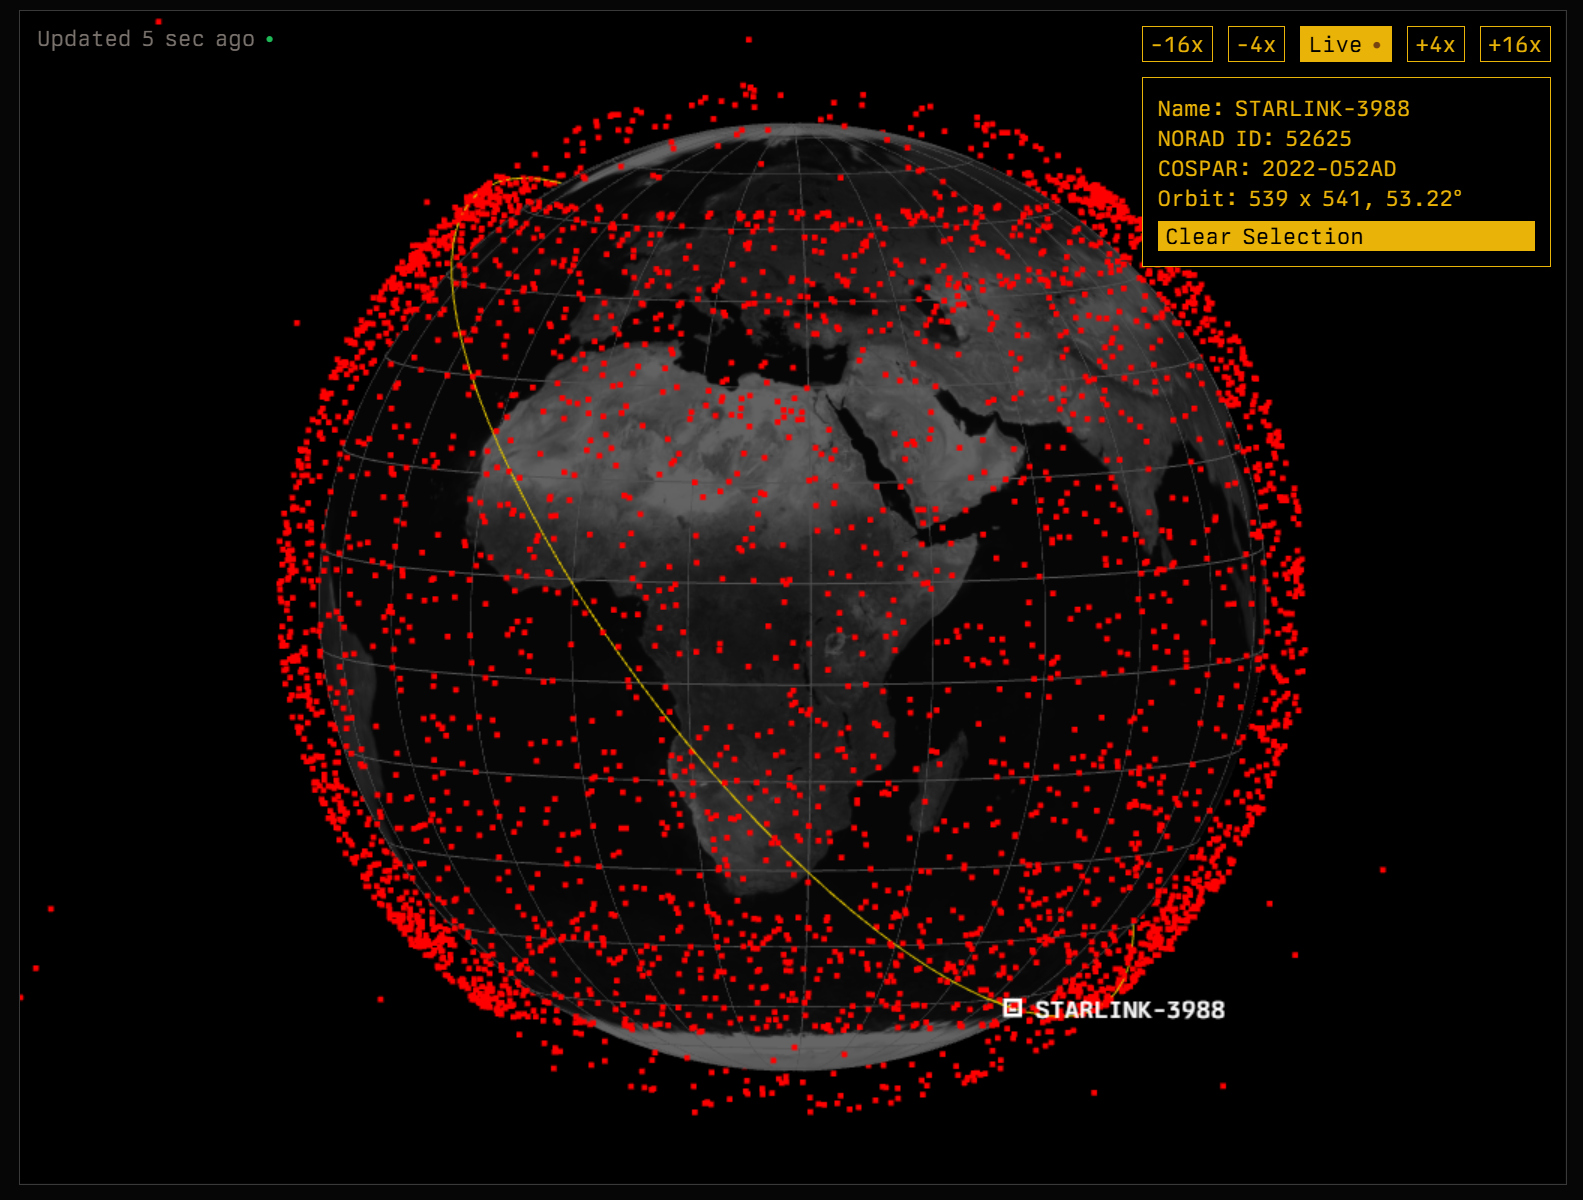
\includegraphics[width=\textwidth]{LaTeX/Figures/Starlink Constellation.png}
    \caption{Starlink constellation as of October 19th 2025, 16:59:33. Each red square represents an active satellite. Highlighted in yellow is the orbital track of selected satellite \textit{Starlink-3988}, with relevant orbital information displayed. The image is a screenshot from the Starlink Map website~\cite{starlinkmap.org}.}
    \label{fig:constellation}
\end{figure}

These satellites have already been used for several key applications, including enabling WiFi connectivity in commercial airlines and cruises, providing life-critical broadband in hurricane-ravaged coastal towns and earthquake-shaken regions, and facilitating allied command and control operations in the Russo-Ukrainian War. The constellation includes nearly 9,700 satellites (as of the writing of this report), and is visualised in Figure~\ref{fig:constellation}. Each unit is equipped with four beamforming, phased array antennas, each of which electronically steers the \SI{11.7}{\giga\hertz} collimated downlink signals in real time to a \SI{24}{\kilo\metre}-diameter ground coverage cell that can serve up to 8,000 simultaneous customers. Furthermore, the satellites communicate with one another via five on-board optical lasers at vacuum light-speed, enabling lower effective latencies between far-away cities compared to underwater cables. This is particularly relevant for applications in stock market trading, where saving a few milliseconds in latency can have a huge impact on the decision-making reactions to market fluctuations. To add to the list of groundbreaking engineering innovations that SpaceX developed for Starlink satellites, the orbital insertion procedure is entirely novel: the satellites are deployed in clusters of up to 23 units\footnote{For the larger v2 model, down from up to 60 units of the smaller v1/v1.5 model} at an altitude of roughly \SI{280}{\kilo\metre}, as shown in Figure~\ref{fig:starlink_cluster}; their orbits are then slowly raised to around \SI{550}{\kilo\metre} in two stages using Kripton gas ion thrusters\footnote{This is a more cost-efficient alternative to the customary option, Xenon gas}. This unusual manoeuvre leaves the satellites bunched up in characteristic lines before successful insertion, which can be observed from the surface of the Earth as shown in Figure~\ref{fig:starlink_line}.

\begin{figure}[h!]
    \centering

    % First subfigure (left image)
    \begin{subfigure}[b]{0.49\textwidth}
        \centering
        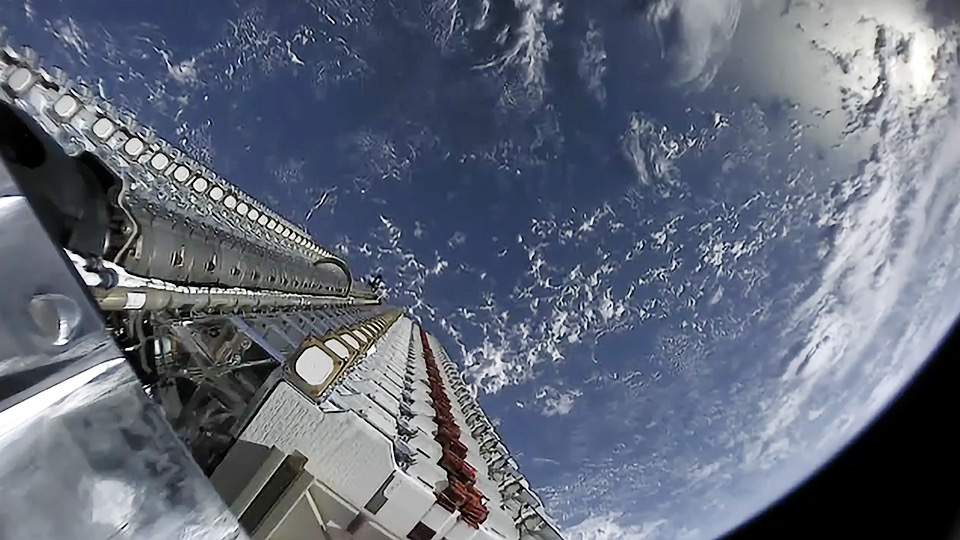
\includegraphics[width=\textwidth]{LaTeX/Figures/Starlink_cluster.jpg}
        \caption{A cluster of Starlink satellites. From~\cite{wikimedia_starlink_mission_2020}.}
        \label{fig:starlink_cluster}
    \end{subfigure}\hfill % No blank line between subfigures
    % Second subfigure (right image)
    \begin{subfigure}[b]{0.49\textwidth}
        \centering
        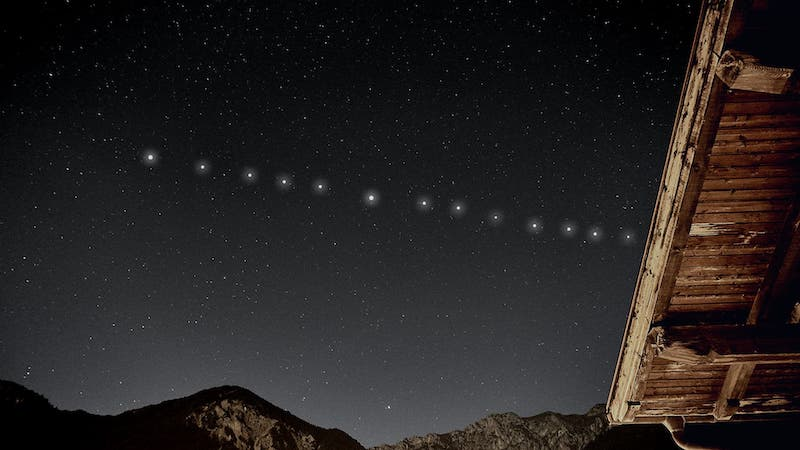
\includegraphics[width=\textwidth]{LaTeX/Figures/SPACEX-STARLINK-SATELLITES-CONSTELLATION.jpeg}
        \caption{A line of Starlink satellites. From~\cite{earthsky_starlink_2021}.}
        \label{fig:starlink_line}
    \end{subfigure}
    
\end{figure}

This project aims to investigate the orbit of an active, Earth-orbiting Starlink satellite through empirical observation and data collection. The satellite chosen is the \textit{Starlink-3988} unit, a v1.5 model as shown in Figure~\ref{fig:satellite_render}: although there aren't any attributes that distinguish it from others in the Starlink constellation, it was selected due to its favourable visibility and consistent orbital passes over Princeton, New Jersey, during the observation window (October 19–22, 2025). Furthermore, the satellite’s low-Earth orbit (LEO) characteristics, including a near-circular path, moderate inclination, and short orbital period, make it ideal for this project's requirements. A detail of the satellite's antennas is shown in Figure~\ref{fig:satellite_antennas}, and relevant attributes are reported in Table~\ref{tab:starlink3988_params}.

\begin{figure}[h!]
    \centering
    
    \begin{subfigure}[b]{0.49\textwidth}
        \centering
        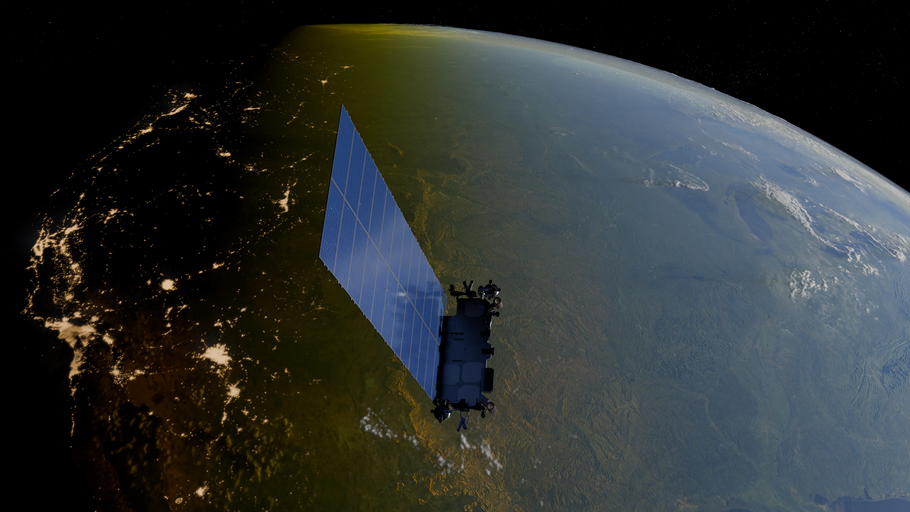
\includegraphics[width=\textwidth]{LaTeX/Figures/satellite_render.png}
        \caption{3D render of a Starlink v1.5 satellite~\cite{wikimedia_starlink_01_2025}.}
        \label{fig:satellite_render}
    \end{subfigure}\hfill
    \begin{subfigure}[b]{0.49\textwidth}
        \centering
        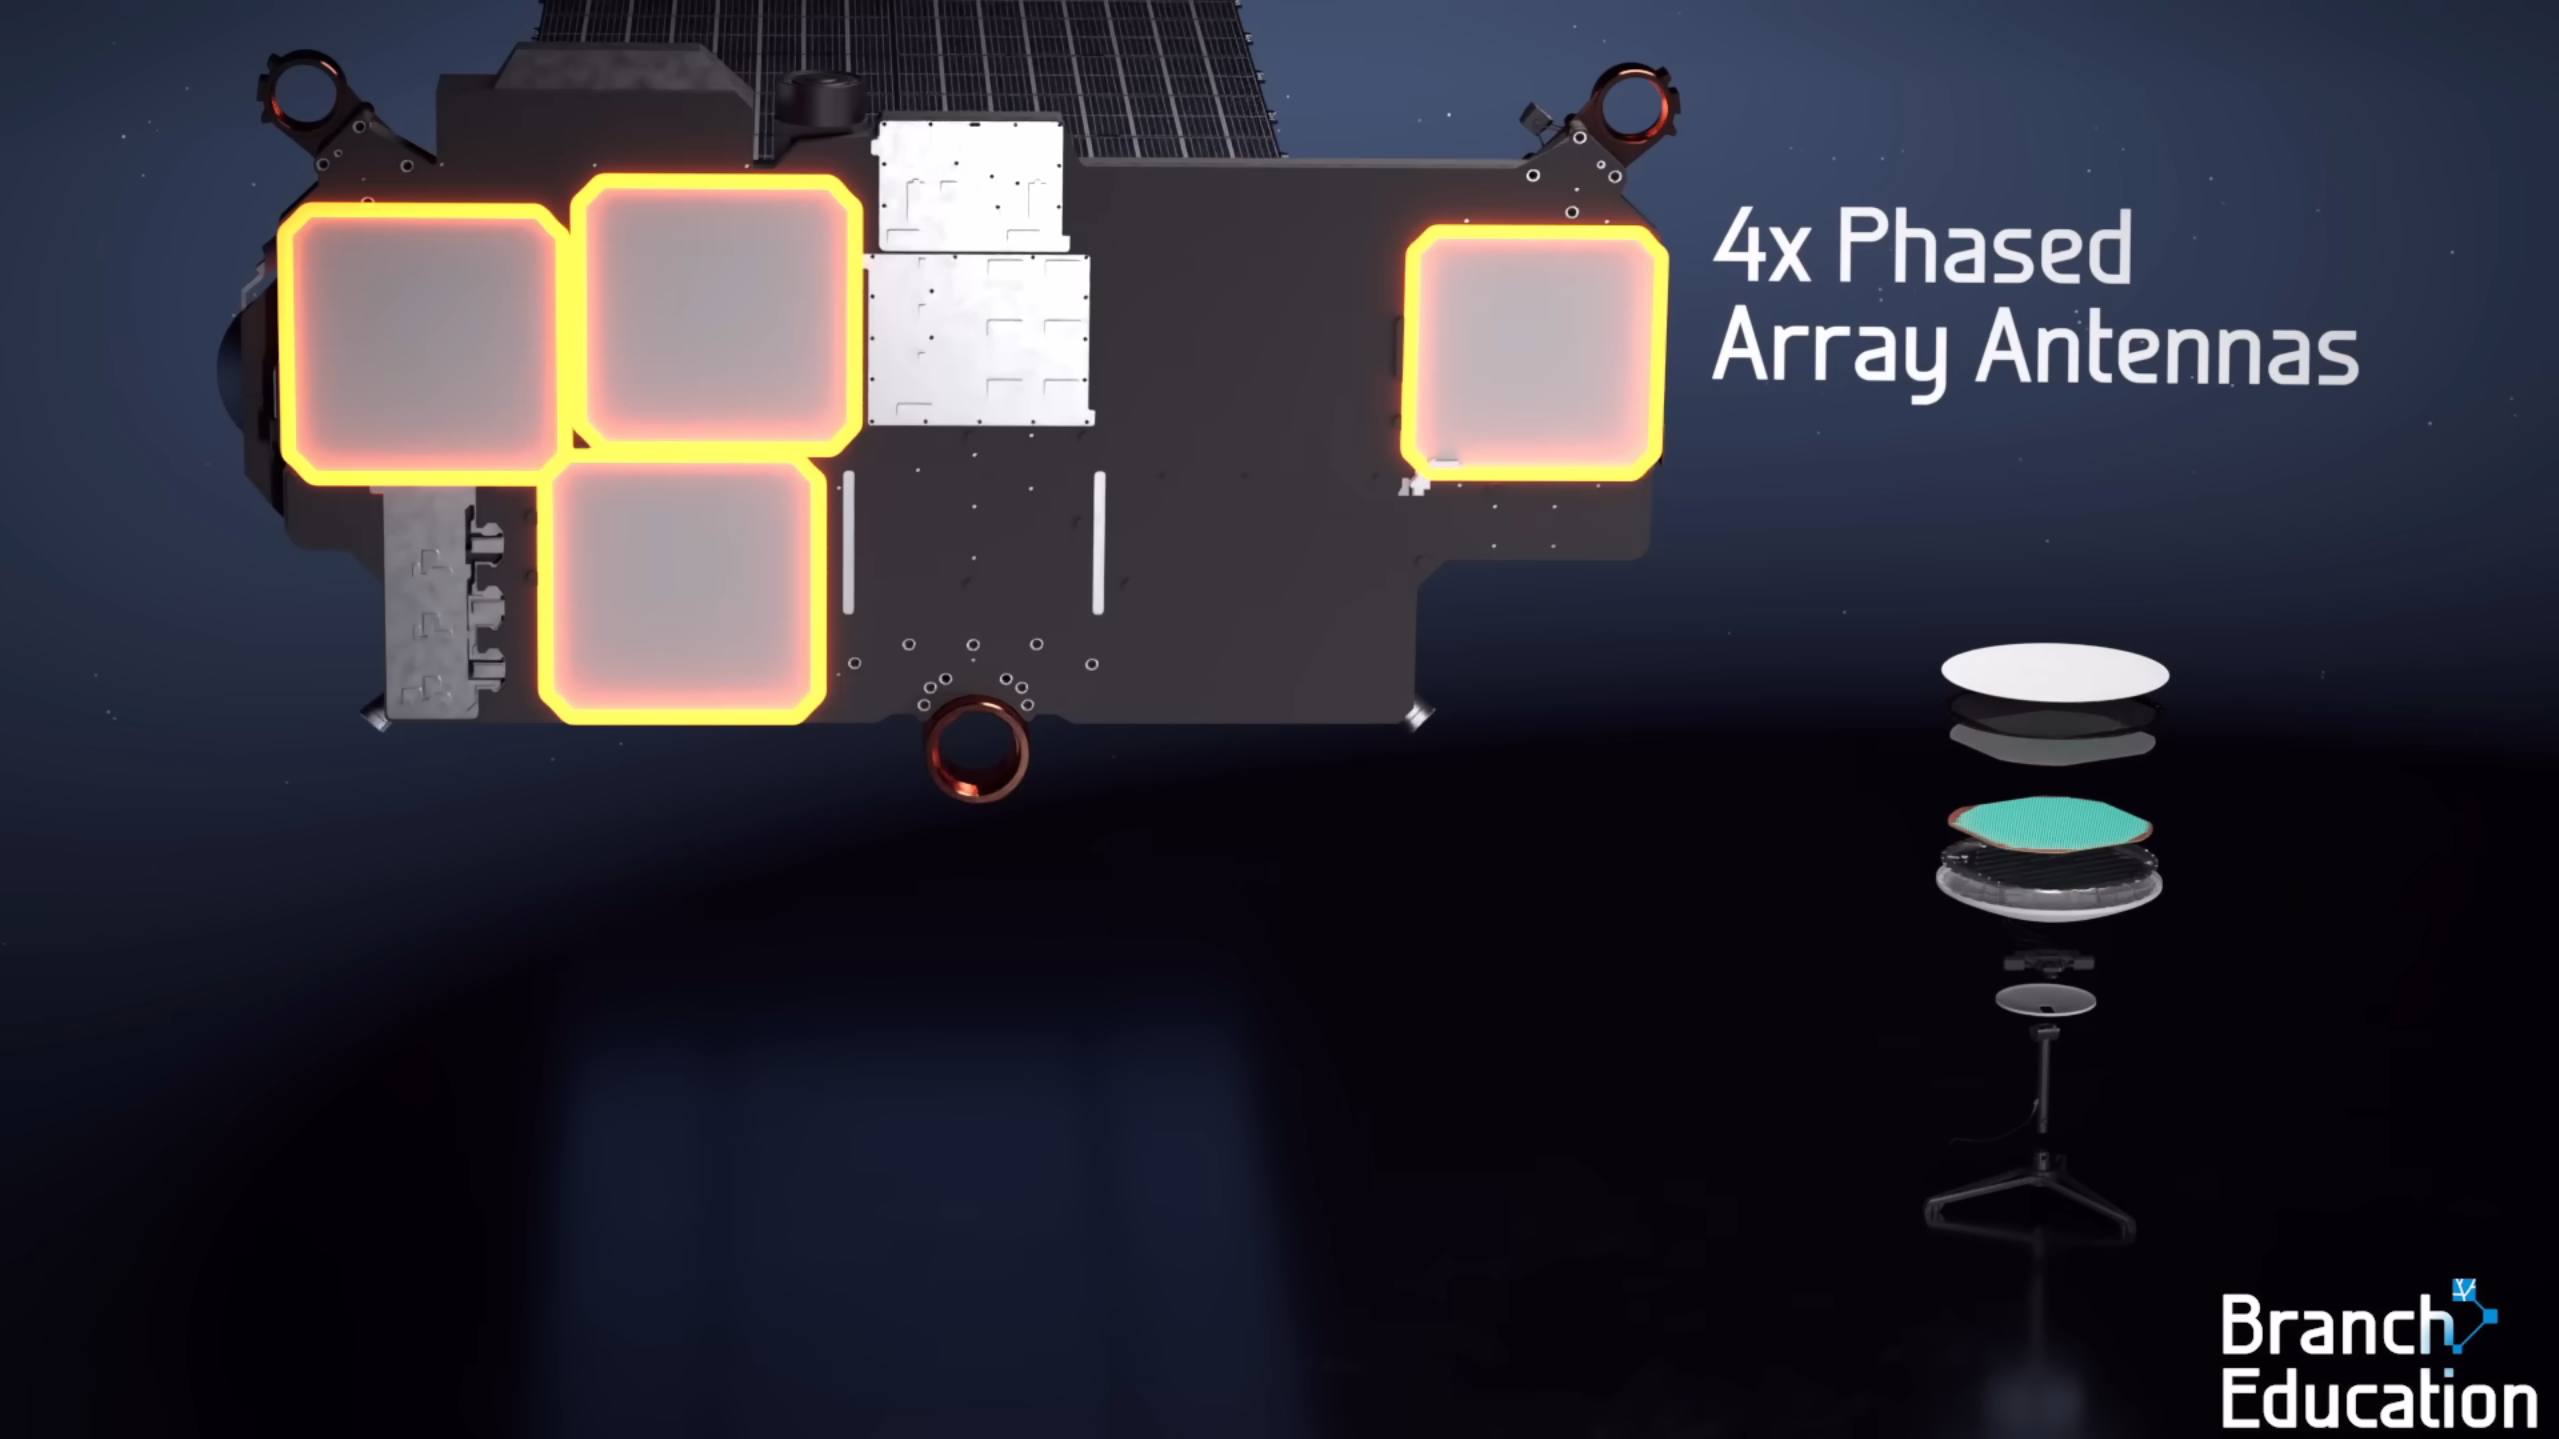
\includegraphics[width=\textwidth]{LaTeX/Figures/satellite_antennas.png}
        \caption{Satellite's antennas and dish. From~\cite{branch_education_starlink_2022}.}
        \label{fig:satellite_antennas}
    \end{subfigure}
    
\end{figure}

\begin{table}[h]
    \centering
    \caption{Identification and physical characteristics of the selected satellite \textit{Starlink-3988}. Data sourced from SpaceX public technical documentation~\cite{spacex_starlink_specs}.}
    \label{tab:starlink3988_params}
    \begin{tabular}{|l|c|}
        \hline
        \textbf{Parameter} & \textbf{Value} \\ \hline
        NORAD Catalog Number & 52625 \\ \hline
        COSPAR ID & 2022-052AD \\ \hline
        Launch Date & May 14, 2022 \\ \hline
        Launch Vehicle / Site & Falcon 9 / Cape Canaveral (AFETR) \\ \hline
        Orbit Type & Low Earth Orbit (LEO) \\ \hline
        Operational Status & Active \\ \hline
        Starlink Model & v1.5 (Laser Inter-satellite Links) \\ \hline
        Dimensions & \SI{2.8}{\metre} $\times$ \SI{1.4}{\metre} $\times$ \SI{0.2}{\metre} (without solar array) \\ \hline
        Mass & 295~\si{\kilogram} \\ \hline
    \end{tabular}
\end{table}

\newpage
\section{Data Collection} \label{sec:data}

To estimate the satellite's orbital period, two different methods were employed:

\begin{enumerate}
    \item Two overhead passes were tracked, with periodic logging of Azimuth and Elevation Angle parameters. In particular, the time of first appearance of the satellite above the horizon, followed by timestamps at every integer minute elapsed, and finally the time of disappearance of the satellite below the horizon, were all recorded. These values were then converted to Right Ascension and Declination, and, using these parameters from two distinct timestamps, the orbital period was estimated. (This corresponds to Method 1 in the instructions provided by the preceptors)
    \item The time at positions of an arbitrarily selected constant elevation angle was recorded, and the orbital period was estimated as an average of these measurements. (This corresponds to Method 4 in the instructions provided by the preceptors)
\end{enumerate}

The results from the two methods were then compared and one of the two results was selected for the remainder of the calculations.

\subsection{Method 1}

The observations of \textit{Starlink-3988} for Method 1 were performed over two separate passes above the Princeton University Art Museum, New Jersey, United States, on 19 October 2025, using a combination of qualitative and quantitative tracking techniques. The \textit{Satellite Tracker} Android application (Vito Technology) was employed for qualitative tracking of the satellite in the night sky. We first used the app to obtain a prediction of the time of appearance of the satellite above the horizon. Then, the app was used to record both the time of appearance and disappearance of the satellite above and below the horizon. On the same Android phone, time was tracked to record the precise moment each integer minute would elapse. Concurrently, the \textit{Satellite Tracker Pro} iOS application (Kornienko Vyacheslav) was used on a separate Apple phone for quantitative measurements. In coordination with time tracking from the Android phone, we logged values of Azimuth and Elevation Angles, as well as the Distance from the observer to the satellite, through consecutive screenshots. By avoiding hand logging the data in real time, the three measurements were simultaneous, and, thus, any potential transient deviation was eliminated. The operation required two mobile phones and two people (the second person involved was the author's roommate, Tomás Consonni, an Economics student who kindly provided access to his iPhone). All times were logged in Eastern Daylight Time (EDT).

The observed Azimuth and Elevation Angles, measured from the Earth's surface, were converted to Right Ascension ($\alpha$) and Declination ($\delta$). This transformation to the equatorial coordinate system, which is relative to the Earth's barycenter, was performed using a \texttt{Python} script provided by the course preceptors. We input the coordinates of our observation station as \SI{40.3463}{\degree}N, \SI{-74.6580}{\degree}E, GMT-04:00. This code also uses the distance to the satellite as an additional input. The raw data are presented in Table~\ref{tab:method1_data} below. Screenshots of the two apps for the very last measurement on the second observation (10/20 at 19:38:16) are displayed in Appendix~\ref{Appendix}.

\begin{table}[H]
    \centering
    \caption{Raw empirical data for Method 1 observations}
    \label{tab:method1_data}
    \renewcommand{\arraystretch}{1.2}
    \begin{tabular}{|c|c|c|c|c|c|c|}
        \hline
        \textbf{Date} & \textbf{Time} & \textbf{Azimuth} & \textbf{Elevation} & \textbf{Distance} & \textbf{Right} & \textbf{Declination} \\ 
        \textbf{(2025)} & \textbf{(EDT)} & \textbf{(°)} & \textbf{Angle (°)} & \textbf{(km)} & \textbf{Ascension (°)} & \textbf{(°)} \\ \hline
        \multicolumn{7}{|c|}{\textbf{Observation 1 – 19 October 2025}} \\ \hline
        10/19 & 21:18:49 & 287.6 & 10.2 & 1628 & 315.8 & 42.8 \\ \hline
        10/19 & 21:19:00 & 286.3 & 11.0 & 1576 & 316.5 & 42.5 \\ \hline
        10/19 & 21:20:00 & 273.1 & 17.9 & 1226 & 321.0 & 39.9 \\ \hline
        10/19 & 21:21:00 & 262.7 & 21.8 & 1083 & 323.4 & 38.5 \\ \hline
        10/19 & 21:22:00 & 241.0 & 26.3 &  954 & 326.5 & 36.3 \\ \hline
        10/19 & 21:23:00 & 213.6 & 25.9 &  541 & 331.7 & 36.5 \\ \hline
        10/19 & 21:24:00 & 190.3 & 20.2 & 1137 & 333.0 & 31.2 \\ \hline
        10/19 & 21:25:00 & 176.0 & 13.7 & 1419 & 336.0 & 28.5 \\ \hline
        10/19 & 21:25:38 & 169.3 & 10.1 & 1657 & 338.0 & 26.5 \\ \hline
        \multicolumn{7}{|c|}{\textbf{Observation 2 – 20 October 2025}} \\ \hline
        10/20 & 19:31:03 & 319.7 & 10.5 & 1636 & 294.0 & 49.7 \\ \hline
        10/20 & 19:32:00 & 325.7 & 17.5 & 1264 & 299.3 & 48.2 \\ \hline
        10/20 & 19:33:00 & 337.5 & 28.0 &  930 & 304.2 & 46.4 \\ \hline
        10/20 & 19:34:00 & 006.1 & 42.2 &  694 & 308.9 & 44.4 \\ \hline
        10/20 & 19:35:00 & 056.7 & 43.7 &  677 & 313.2 & 42.2 \\ \hline
        10/20 & 19:36:00 & 088.6 & 29.9 &  886 & 317.2 & 39.9 \\ \hline
        10/20 & 19:37:00 & 101.9 & 18.6 & 1216 & 321.0 & 37.4 \\ \hline
        10/20 & 19:38:00 & 108.3 & 11.3 & 1579 & 324.4 & 34.9 \\ \hline
        10/20 & 19:38:16 & 109.5 & 09.8 & 1675 & 325.3 & 34.3 \\ \hline
    \end{tabular}
\end{table}

In preparation for the real observation, a test logging of data was also performed using the \textit{In The Sky} website. These data can be found in Appendix~\ref{Appendix} and do not contain distance to satellite entries.

\subsection{Method 4}

For the implementation of Method 4, we employed a similar experimental setup. Observations were conducted from Princeton University Art Museum, New Jersey, United States, during the 20th and 21st of October 2025.

\begin{table}[H]
    \centering
    \caption{Raw empirical data for Method 4 observations}
    \label{tab:method4_data}
    \renewcommand{\arraystretch}{1.2}
    \begin{tabular}{|c|c|c|c|c|}
        \hline
        \textbf{Date (2025)} & \textbf{Time (EDT)} & \textbf{Elevation Angle (°)} & \textbf{Latitude (°N)} & \textbf{Longitude (°E)} \\ \hline
        \multicolumn{5}{|c|}{\textbf{Observations – 21 October 2025}} \\ \hline
        10/20 & 15:10:29 & -80.0 & -43.63 & 79.67\\ \hline
        10/20 & 16:49:20 & -80.0 & -58.24 & 72.31\\ \hline
        10/20 & 18:27:27 & -80.0 & -63.85 & 73.79\\ \hline
        10/21 & 16:59:42 & -80.0 & -48.42 & 129.85\\ \hline
        10/21 & 18:40:59 & -80.0 & -35.67 & 128.85\\ \hline
        10/21 & 20:24:44 & -80.0 & -23.76 & 116.68 \\ \hline
    \end{tabular}
\end{table}


 The \textit{N2YO} website (\href{https://www.n2yo.com}{https://www.n2yo.com}) was employed for quantitative tracking: we screen-recorded a portion of the website containing data about time, Elevation Angle, latitude and longitude over several hours of time on two separate days. The recorded footage was later analysed to extract precise timestamps at which the satellite crossed a constant elevation angle during each pass. By employing this technique, a consistent dataset was obtained without the need for manual data entry, thereby reducing human timing errors. An example screenshot of the data obtained from the screen recording is displayed in Appendix~\ref{Appendix}. All times were recorded in Eastern Daylight Time (EDT). The elapsed times between consecutive passes at the same elevation will be used to estimate the orbital period. The raw data are summarised in Table~\ref{tab:method4_data}.

\section{Estimate of Period and Angular Velocity}

The purpose of this section is to calculate orbital period and angular velocity for the \textit{Starlink-3988} satellite using the data presented in Section~\ref{sec:data}. All calculations were performed using \texttt{Python}, and scripts can be found at the supporting repository:
\begin{center}
    \href{https://github.com/ClouD-161803/MAE341-Project1}{ClouD-161803/MAE341-Project1}.
\end{center}

To carry out the calculations below, we made several simplifying assumptions:

\begin{itemize}
    \item The mass of the satellite is negligible when compared to that of the Earth, so the Earth remains stationary whilst the satellite is orbiting it.
    \item The orbital influence of any perturbations to the two-body problem, including gravitational field distortions due to Earth's shape, atmospheric drag, lunisolar perturbations, and solar radiation pressure, was assumed to be negligible and was not accounted for in our methods.
    \item For processing data emanating from Method 1 collection, we assumed the orbital path traced by the satellite is a perfect circle. This assumption implies that the true anomaly and the eccentric anomaly are equal at all times. We will show the validity of this assumption when evaluating the (elliptical) orbit's eccentricity, and show that it is very close to the assumed value of $0$. As a result, the satellite is assumed to be travelling in a straight line on the surface of a 2-sphere (whose radius is the orbital radius, i.e. Earth's radius plus altitude). This path is also known as a geodesic.
    \item For processing data emanating from Method 4 collection, we assumed that the satellite completes a full orbit when crossing the same elevation angle at two separate times. Note that the condition to be met is that both the elevation angle's value \emph{and} the sign of its rate of change (positive for ascension, negative for descent) are equal. It is noted that, within each orbit, the satellite passes a given elevation angle \emph{twice}, once on ascent and once on descent. We were careful to consider the descent timestep for each orbital pass. 
\end{itemize}

The following constants were used throughout for numerical evaluation of all parameters:

\begin{center}
    \vspace{0.5em}
    
    \begin{tabular}{l c}
        Earth gravitational parameter & $\mu_{\text{E}} = \SI{398574}{\kilo\meter^3\per\second^2}$ \\[0.3em]
        Mean radius of Earth & $R_{\text{E}} = \SI{6378}{\kilo\meter}$ \\[0.3em]
        Mass of Earth & $M_{\text{E}} = \SI{5.9722e24}{\kilogram}$ \\[0.3em]
    \end{tabular}
\end{center}

\subsection{Orbital Period}

\subsubsection{Method 4}

Using Method~4, the orbital period is determined from the elapsed time between successive appearances of the satellite at a fixed elevation angle. Our selection of angle fell on an elevation angle of $-80^{\circ}$ (for no particular reason). By computing the time interval between successive passes of identical elevation, the orbital period $\tau$ can be estimated directly as the difference in observation times. The resulting orbital periods for each consecutive pass are presented in Table~\ref{tab:method4_periods}. The intervals were converted to minutes and compared with the published value ($\tau_{\text{true}} = \SI{95.4}{\minute}$).

\begin{table}[H]
    \centering
    \caption{Orbital period estimates using Method~4 (constant elevation angle).}
    \label{tab:method4_periods}
    \renewcommand{\arraystretch}{1.2}
    \begin{tabular}{|c|c|c|c|}
        \hline
        \textbf{Pass Interval} & \textbf{Time Difference (hh:mm:ss)} & \textbf{$\tau$ (\si{\minute})} & \textbf{Error vs. True (\%)} \\ \hline
        1–2 & 01:38:51 & 98.85 & +3.61 \\ \hline
        2–3 & 01:38:07 & 98.12 & +2.84 \\ \hline
        4–5 & 01:41:17 & 101.28 & +6.15 \\ \hline
        5–6 & 01:43:45 & 103.75 & +8.73 \\ \hline
        \textbf{Mean} &  & \textbf{100.00} & \textbf{+4.81} \\ \hline
    \end{tabular}
\end{table}

From Table~\ref{tab:method4_periods}, the mean orbital period obtained via Method~4 was $\bar{\tau}_{4} = \SI{100.0}{\minute}$, which exceeds the true period by approximately \SI{4.8}{\percent}. This systematic overestimation likely stems from the relatively coarse time resolution of the available constant-elevation data and potential timing offsets in the dataset. Moreover, Method~4 is sensitive to local geometric distortions in elevation tracking and assumes perfectly consistent ground geometry between passes, which is likely not achieved in practice as the satellite's position above the Earth changes with each orbit (notice the drift in Latitude and Longitude from Table~\ref{tab:method4_data}). Therefore, although Method~4 provides a reasonable first-order estimate, its reliance on single-point elevation measurements introduces significant temporal and geometric uncertainty. The method is simple to apply when constant-elevation crossings are clearly recorded, but it is be vulnerable to several sources of error.

\subsubsection{Method 1}

Using Method 1, we calculated several pairs of Right Ascension ($\alpha$) and Declination ($\delta$) coordinates. The selected data points for the calculations following correspond to the Second Observation half of Table~\ref{tab:method1_data}. For two consecutive observations of the satellite separated by a known time interval $\Delta t$, the angular displacement $\psi$ on the celestial sphere is approximated using the arc of geodesic separating the two points:

\[
    \cos{\psi} = \sin{\delta_1}\sin{\delta_2} + \cos{\delta_1}\cos{\delta_2}\cos{(\alpha_2 - \alpha_1)}.
    \label{eq:psi_equation}
\]

The corresponding angular distance $\psi$ (in radians) is then:

\begin{equation}
    \psi = \cos^{-1}\!\left[\sin{\delta_1}\sin{\delta_2} + \cos{\delta_1}\cos{\delta_2}\cos{(\alpha_2 - \alpha_1)}\right].
    \label{eq:psi_angle}
\end{equation}

For a circular orbit, the orbital period $\tau$ can be estimated from the total angular displacement of $2\pi$ radians over one revolution, rearranging the relation between $\psi$, $\Delta t$, and $\tau$ as follows:

\begin{equation}
    \tau = \frac{2\pi\,\Delta t}{\psi}.
    \label{eq:tau_from_psi}
\end{equation}

Several pairs of observations were selected from the Second Observation session of Table~\ref{tab:method1_data} (10/20/2025) to evaluate the consistency of the result. The values of $\psi$, angular velocity $\omega$ were computed in a parallel fashion using~\eqref{eq:psi_angle}, and the resulting period $\tau$ with~\eqref{eq:tau_from_psi}. The results are summarised in Table~\ref{tab:psi_periods}, and plotted in Figure~\ref{fig:psi_periods_plot}.

\begin{table}[H]
    \centering
    \caption{Orbital period estimates using Method~1 for various right ascension/declination pairs from Observation 2 (10/20) of Method 1.}
    \label{tab:psi_periods}
    \renewcommand{\arraystretch}{1.15}
    \begin{tabular}{|c|c|c|c|c|}
        \hline
        \textbf{Pair} & $\Delta t$ (\si{\second}) & $\psi$ (\si{\degree}) & $\omega$ (\si{\degree\per\second}) & $\tau$ (\si{\minute}) \\ \hline
        1--5 & 237 & 15.2228 & 0.064231 & 93.41 \\ \hline
        2--6 & 240 & 15.2429 & 0.063512 & 94.47 \\ \hline
        3--7 & 240 & 15.2914 & 0.063714 & 94.17 \\ \hline
        4--8 & 240 & 15.1641 & 0.063184 & 94.96 \\ \hline
        1--6 & 297 & 19.0336 & 0.064086 & 93.62 \\ \hline
        2--7 & 300 & 19.1123 & 0.063708 & 94.18 \\ \hline
        3--8 & 300 & 19.0354 & 0.063451 & 94.56 \\ \hline
        1--7 & 357 & 22.9031 & 0.064154 & 93.53 \\ \hline
        2--8 & 360 & 22.8563 & 0.063490 & 94.50 \\ \hline
        1--8 & 417 & 26.6471 & 0.063902 & 93.89 \\ \hline
    \end{tabular}
\end{table}

From the ten independent estimates in Table~\ref{tab:psi_periods}, the mean period and standard deviation were computed as:
\[
\bar{\tau} = \SI{94.13}{\minute}, \qquad \sigma_\tau = \SI{0.50}{\minute}.
\]
These results exhibit strong consistency across all selected pairs, with less than \SI{1}{\minute} of spread.  
The small scatter reflects good internal precision but does not include potential systematic uncertainties, such as timing offsets, coordinate conversion accuracy, or deviations from the circular orbit assumption.

\begin{figure}[H]
    \centering
    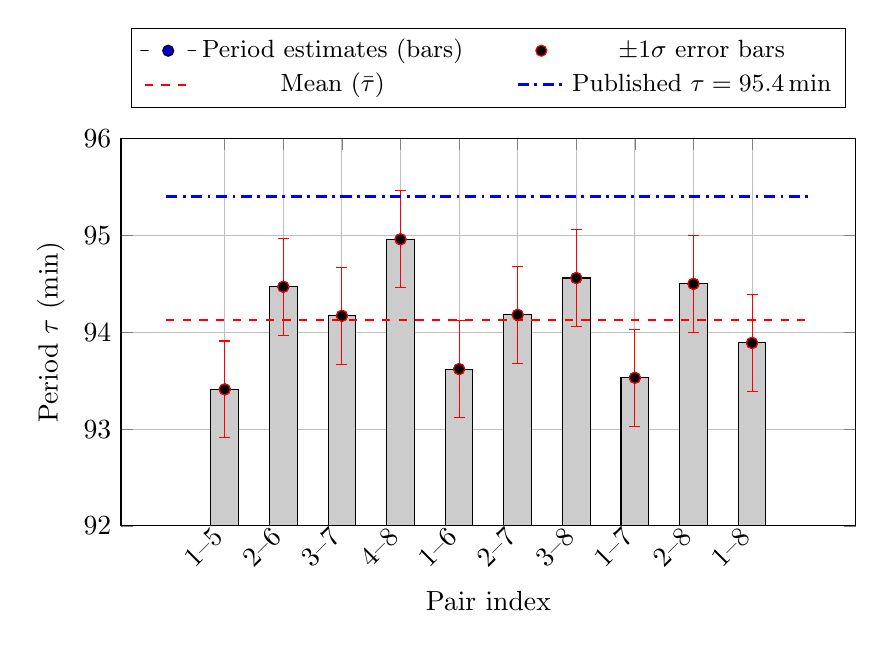
\begin{tikzpicture}
        \begin{axis}[
            width=0.9\linewidth,
            height=6.5cm,
            xlabel={Pair index},
            ylabel={Period $\tau$ (\si{\minute})},
            ymin=92, ymax=96,
            xtick={1,...,10},
            xticklabels={1--5,2--6,3--7,4--8,1--6,2--7,3--8,1--7,2--8,1--8},
            x tick label style={rotate=45, anchor=east},
            grid=major,
            bar width=10pt,
            enlarge x limits=0.07,
            legend style={
                at={(0.5,1.08)},
                anchor=south,
                draw=black,
                fill=white,
                font=\small,
                legend columns=2,
                /tikz/every even column/.append style={column sep=0.6cm}
            }
        ]
        % Bar chart of the period estimates
        \addplot+[ybar, fill=gray!40, draw=black] coordinates {
            (1,93.41) (2,94.47) (3,94.17) (4,94.96) (5,93.62)
            (6,94.18) (7,94.56) (8,93.53) (9,94.50) (10,93.89)
        };
        % Error bars (±1 sigma) as black markers with error bars
        \addplot+[only marks, mark=*, mark options={fill=black}, error bars/.cd, y dir=both, y explicit]
        coordinates {
            (1,93.41) +- (0,0.50)
            (2,94.47) +- (0,0.50)
            (3,94.17) +- (0,0.50)
            (4,94.96) +- (0,0.50)
            (5,93.62) +- (0,0.50)
            (6,94.18) +- (0,0.50)
            (7,94.56) +- (0,0.50)
            (8,93.53) +- (0,0.50)
            (9,94.50) +- (0,0.50)
            (10,93.89) +- (0,0.50)
        };
        % Mean line (dashed red)
        \addplot [red, thick, dashed] coordinates {(0,94.13) (11,94.13)};
        % Published / stated value line (dot-dashed blue)
        \addplot [blue, very thick, dash pattern=on 4pt off 2pt on 1pt off 2pt] coordinates {(0,95.40) (11,95.40)};
        % Legend (two columns, two rows)
        \legend{
            Period estimates (bars),
            $\pm1\sigma$ error bars,
            Mean ($\bar{\tau}$),
            Published $\tau=95.4\,$min
        }
        \end{axis}
    \end{tikzpicture}
    \caption{Orbital period estimates for each observation pair: bars show individual estimates, black markers with error bars indicate $\pm1\sigma$ uncertainty, the dashed red line represents the mean estimate ($\bar{\tau}=\SI{94.13}{\minute}$), and the blue dot-dashed line marks the published value ($\tau=\SI{95.4}{\minute}$).}
    \label{fig:psi_periods_plot}
\end{figure}

Taking the mean value $\bar{\tau} = \SI{94.13}{\minute}$ as the best estimate for the orbital period and comparing it with the published value of \SI{95.4}{\minute}~\cite{n2yo_starlink3988}, the percentage error is
\[
\varepsilon = \frac{|\bar{\tau} - \tau_\text{true}|}{\tau_\text{true}} \times 100
           = \frac{|94.13 - 95.4|}{95.4} \times 100 = \SI{1.33}{\percent}.
\]

We noted that all of the measurements involving index~1 were systematically below the empirical mean value, often outside of the $1\sigma$ range. This points to a likely human error in the measurement of the first timestamp for the second observation. To refine the estimate, we removed all pairs containing index~1 from the dataset and recomputed the mean and standard deviation, plotting the results in Figure~\ref{fig:psi_periods_refined}. The recalculated statistics were:
\[
\bar{\tau}_{\text{refined}} = \SI{94.47}{\minute}, \qquad \sigma_{\tau,\text{refined}} = \SI{0.46}{\minute}.
\]

\subsubsection{Comparison}

Method~4 produced a mean $\bar{\tau}_{4}=\SI{100.0}{\minute}$ (error vs.\ published value of +\SI{4.8}{\percent}), whereas the refined Method~1 result is $\bar{\tau}_{\text{refined}}=\SI{94.47}{\minute}$ (error vs.\ published value of \SI{0.97}{\percent}). Method~1 therefore yields both a closer agreement with the published orbital period and a much smaller internal scatter (after removing the identified systematic involving index~1). Method~4 is straightforward to apply when constant-elevation events are reliably recorded, but it is more vulnerable to timing bias, mis-identification of passes, and projection/geometric effects. Method~1 requires more processing (coordinate transformations and pairwise angular calculations) but benefits from averaging many angular separations on the celestial sphere and is less sensitive to a single erroneous timestamp, and hence is more reliable. Therefore, we chose the results of Method 1.

\begin{figure}[h]
    \centering
    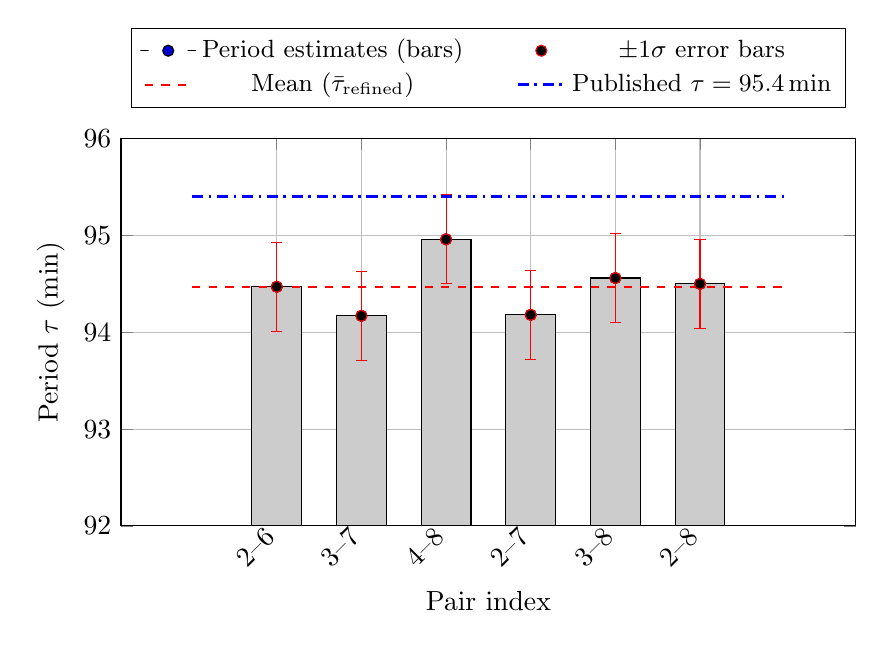
\begin{tikzpicture}
        \begin{axis}[
            width=0.9\linewidth,
            height=6.5cm,
            xlabel={Pair index},
            ylabel={Period $\tau$ (\si{\minute})},
            ymin=92, ymax=96,
            xtick={1,...,6},
            xticklabels={2--6,3--7,4--8,2--7,3--8,2--8},
            x tick label style={rotate=45, anchor=east},
            grid=major,
            bar width=18pt,
            enlarge x limits=0.12,
            legend style={
                at={(0.5,1.08)},
                anchor=south,
                draw=black,
                fill=white,
                font=\small,
                legend columns=2,
                /tikz/every even column/.append style={column sep=0.6cm}
            }
        ]
        % Bar chart of the refined period estimates (pairs without index 1)
        \addplot+[ybar, fill=gray!40, draw=black] coordinates {
            (1,94.47) (2,94.17) (3,94.96) (4,94.18) (5,94.56) (6,94.50)
        };
        % Error bars (±1 sigma, refined) as black markers with error bars, superimposed
        \addplot+[only marks, mark=*, mark options={fill=black}, error bars/.cd, y dir=both, y explicit]
        coordinates {
            (1,94.47) +- (0,0.46)
            (2,94.17) +- (0,0.46)
            (3,94.96) +- (0,0.46)
            (4,94.18) +- (0,0.46)
            (5,94.56) +- (0,0.46)
            (6,94.50) +- (0,0.46)
        };
        % Refined mean line (dashed red)
        \addplot [red, thick, dashed] coordinates {(0,94.47) (7,94.47)};
        % Published / stated value line (dot-dashed blue)
        \addplot [blue, very thick, dash pattern=on 4pt off 2pt on 1pt off 2pt] coordinates {(0,95.40) (7,95.40)};
        % Legend (two columns)
        \legend{
            Period estimates (bars),
            $\pm1\sigma$ error bars,
            Mean ($\bar{\tau}_{\mathrm{refined}}$),
            Published $\tau=95.4\,$min
        }
        \end{axis}
    \end{tikzpicture}
    \caption{Refined orbital period estimates (pairs excluding index~1). Bars show individual estimates, black markers with error bars indicate $\pm1\sigma$ uncertainty (using the refined $\sigma_{\tau}=\SI{0.46}{\minute}$), the dashed red line represents the refined mean ($\bar{\tau}_{\mathrm{refined}}=\SI{94.47}{\minute}$), and the blue dot-dashed line marks the published value ($\tau=\SI{95.4}{\minute}$).}
    \label{fig:psi_periods_refined}
\end{figure}

\subsection{Angular Velocity}

Keeping index~1 excluded from the dataset, we also computed the corresponding mean angular velocity, defined as \[ \omega = \frac{2\pi}{\tau}. \] Using the refined mean orbital period $\bar{\tau}_{\text{refined}} = \SI{94.47}{\minute}$, the resulting mean angular velocity is \[ \bar{\omega}_{\text{refined}} = \frac{2\pi}{94.47\times60} = \SI{0.001108}{\radian\per\second} = \SI{0.06347}{\degree\per\second}. \] The uncertainty in $\omega$ measurement arises from the propagation of the period uncertainty, $\sigma_{\tau,\text{refined}} = \SI{0.46}{\minute}$, through the inverse relationship $\omega \propto 1/\tau$, and is also very small, indicating internal consistency.

We adopt the refined values from Method~1,
\[
    \bar{\tau}_{\text{refined}} = \SI{94.47}{\minute}, \qquad 
    \bar{\omega}_{\text{refined}} = \SI{1.108e-3}{\radian\per\second},
\]
as the definitive parameters for all subsequent orbital calculations in this report.

\section{Estimate of Semi-Major Axis and Position Prediction}

The remainder of this report is concerned with the evaluation of orbital elements for the orbit of the \textit{Starlink-3988} satellite. In general, orbital elements are a set of parameters that fully define the shape of a satellite's orbit around a central body, as well as the position of the satellite along the orbit, effectively nailing the location of the satellite in 3D space at a given time relative to a given reference frame. The most common set of orbital parameters to describe orbits of satellites around the Earth is that of the six orbital elements: eccentricity ($e$), semi-major axis ($a$), inclination ($i$), longitude of the ascending node ($\Omega$), argument of periapsis ($\omega$), and true anomaly ($\theta$). For reference and comparison, the ground truth TLE values for the \textit{Starlink-3988} satellite are given in Table~\ref{tab:starlink3988_orbit}. These were taken from the \textit{N2YO} website, and a full explanation of how we converted the raw TLEs to the values in the table is given in Appendix~\ref{AppendixB}. In this section, we will evaluate the semi-major axis, and carry out a point prediction of the position of the satellite in the future, and compare our results to the ground truth values from Table~\ref{tab:starlink3988_orbit}.

\begin{table}[h]
    \centering
    \caption{Orbital parameters for \textit{Starlink-3988}. Data sourced from N2YO~\cite{n2yo_starlink3988} at 18:53:19~EDT.}
    \label{tab:starlink3988_orbit}
    \begin{tabular}{|l|c|c|}
        \hline
        \textbf{Parameter} & \textbf{Symbol / Unit} & \textbf{TLE Value} \\ \hline
        Date & $(YYYY-MM-DD)$ & 2025-10-21 \\ \hline
        Epoch (UTC) & $(hh:mm:ss)$ & 22:53:19 \\ \hline
        Inclination & $i$ (\si{\degree}) & 53.2146 \\ \hline
        Right Ascension of Ascending Node & $\Omega$ (\si{\degree}) & 171.9324 \\ \hline
        Eccentricity & $e$ () & 0.0001133 \\ \hline
        Argument of Perigee & $\omega$ (\si{\degree}) & 95.0058 \\ \hline
        Semi-Major Axis & $a$ (\si{\kilo\metre}) & 6917 \\ \hline
        Mean Anomaly & $M$ (\si{\degree}) & 265.1064 \\ \hline
        Perigee Altitude & $h_p$ (\si{\kilo\metre}) & 545.9 \\ \hline
        Apogee Altitude & $h_a$ (\si{\kilo\metre}) & 547.9 \\ \hline
        Mean Altitude & $h$ (\si{\kilo\metre}) & 546.9 \\ \hline
        Orbital Period & $\tau$ (\si{\minute}) & 95.43 \\ \hline
        Mean Motion & $n$ (\si{rev/day}) & 15.088489 \\ \hline
    \end{tabular}
\end{table}

\subsection{Semi-Major Axis}

The semi-major axis of a satellite's closed elliptical orbit refers to half the distance that separates the point of closest approach to the centre of the Earth (perigee) to that of furthest distance away (apogee). Naturally, it has dimensions of length. From Kepler's third law, the semi-major axis is related to the orbital period via:

\[
\tau^{2} = \frac{4\pi^{2}}{\mu} a^{3},
\]
where $\mu$ is Earth's standard gravitational parameter.  
Rearranging for $a$ gives:
\begin{equation}
\label{semi_major_axis_from_tau}
    a = \left( \frac{\mu \tau^{2}}{4\pi^{2}} \right)^{1/3}.
\end{equation}

Using the refined orbital period obtained previously of $\bar{\tau} = \SI{94.47}{\minute}$, which corresponds to:
\[
\bar{\tau} = \SI{94.47}{\minute} \times \SI{60}{\second\per\minute} = \SI{5668}{\second},
\]
we substitute into~\eqref{semi_major_axis_from_tau}:
\[
\bar{a} = \left( \frac{(\SI{398574}{\kilo\metre^{3}\per\second^{2}}) (\num{3.215e7})}{\num{39.478}} \right)^{1/3}
   = \left( \num{3.246e11} \right)^{1/3}.
\]
Hence:
\[
\boxed{\bar{a} = \SI{6938}{\kilo\metre}},
\]
to four significant figures.

Since the orbit was assumed to be circular (we will show this is a good assumption in Section~\ref{sec:orbital_elements}), the computed semi-major axis of $\bar{a} = \SI{6938}{\kilo\metre}$ also corresponds to the mean orbital radius of the satellite.  
For comparison, the semi-major axis derived from the satellite’s published orbital elements (Two-Line Element set, TLE) given in Table~\ref{tab:starlink3988_orbit} is:
\[
a_{\text{TLE}} = \SI{6917}{\kilo\metre}.
\]
The difference between the observed and tabulated values is therefore:
\[
\Delta a = \bar{a} - a_{\text{TLE}} = \SI{21}{\kilo\metre},
\]
corresponding to a relative error of:
\[
\frac{|\Delta a|}{a_{\text{TLE}}} \times 100 = \SI{0.30}{\percent}.
\]
This small deviation is well within experimental uncertainty and primarily arises from limited precision in the timing of orbital passes, as well as the simplifying assumption of a perfectly circular orbit ($e \approx 0$), which neglects the satellite’s small but nonzero eccentricity.

\subsection{Position Prediction via Kepler’s Equation}

Having determined the orbital period $\tau$ and semi-major axis $a$, we can predict the satellite’s position along its orbit at any future time using Kepler’s equation:
\begin{equation}
    \label{eq:kepler_equation}
    M_e = \varepsilon_e - e\sin \varepsilon_e,
\end{equation}
where $M_e$ is the elliptical mean anomaly and $\varepsilon_e$ is the elliptical eccentric anomaly. For small eccentricities this relation simplifies to $M_e \approx \varepsilon_e \approx \theta$, where $\theta$ denotes the true anomaly. Choosing a reference time $t_0$ corresponding to a known satellite position, the mean anomaly at a later time $t$ is given by:
\[
M_e(t) = \frac{2\pi}{\tau}(t - t_0).
\]
Substituting $M_e$ into~\eqref{eq:kepler_equation} requires an iterative solution for $\varepsilon_e$ (examples of numerical schemes are bisection or Newton's method). The radius vector is then:
\[
r = a(1 - e\cos \varepsilon_e),
\]
and the true anomaly may be recovered from the geometry of the ellipse. For circular orbits ($e \approx 0$) the computation simplifies significantly:
\[
\theta(t) = M_e(t) = \frac{2\pi}{\tau}(t - t_0).
\]
This allows direct prediction of the satellite’s angular position and corresponding ground track as a function of elapsed time. To evaluate a point prediction, we therefore need a starting time, with known value of mean anomaly, and a prediction window $t - t_0$ to evaluate against. 

\begin{figure}[h]
    \centering
    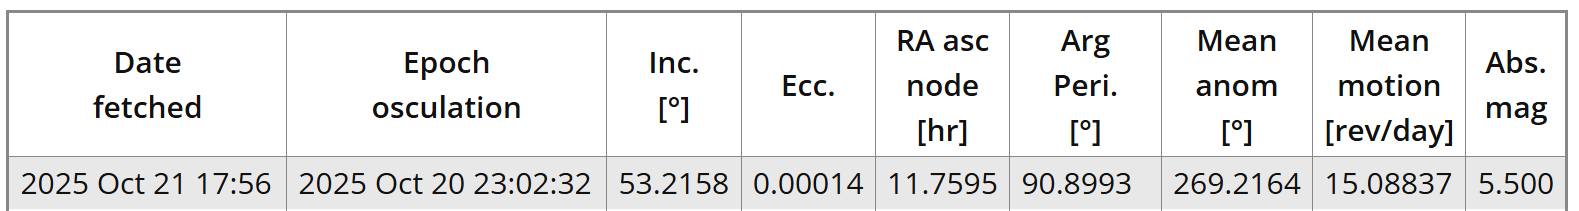
\includegraphics[width=\textwidth]{LaTeX/Figures/TLE_from_in_the_sky.png}
    \caption{Screenshot of the \textit{Starlink-3988} TLE as fetched from the \textit{In-The-Sky} website.}
    \label{fig:inthesky_tle}
\end{figure}

The choice of initial time was dictated by the availability of TLEs from online sources. The closest TLE we could obtain to our measurement timestamps was for 2025-10-20 at 23:02:32 UTC, which is very close to the measurement on the first row of Observation 2 in Table~\ref{tab:method1_data} (2025-10-20 at 19:31:03 EDT or 23:31:03 UTC, i.e. 28 minutes and 31 seconds before the satellite rose over the horizon at our location). This TLE was obtained from the \textit{In-The-Sky} website, a screenshot of which is given in Figure~\ref{fig:inthesky_tle}. The mean anomaly reported at this osculation epoch is \(M_{0}=\SI{269.2164}{\degree}\). The target time is that of the TLE of Table~\ref{tab:starlink3988_orbit}, namely \(t=\) 2025-10-21 18:53:19 EDT \(=\) 2025-10-21 22:53:19 UTC. The elapsed time is therefore:
\[
\Delta t = t - t_{0}
= \text{2025-10-21 22:53:19 UTC} - \text{2025-10-20 23:02:32 UTC}
= \SI{85847}{\second}.
\]
Using the observational estimate \(\bar{\tau}=\SI{94.47}{\minute}=\SI{5668.2}{\second}\) to propagate mean anomaly forward, the number of revolutions during \(\Delta t\) is:
\[
\Delta N = \frac{\Delta t}{\bar{\tau}}
= \frac{\SI{85847}{\second}}{\SI{5668.2}{\second}}
= \num{15.14537243}\ \text{revolutions},
\]
which corresponds to an angular advance of:
\[
\Delta M = 360^\circ\,\Delta N
= 360^\circ\times\num{15.14537243}
= \SI{5452.3341}{\degree}.
\]
Adding this advance to the initial mean anomaly gives:
\[
\bar{M}_{e} = M_{0} + \Delta M
= \SI{269.2164}{\degree} + \SI{5452.3341}{\degree}
= \SI{5721.5505}{\degree}.
\]
Reduced to the principal range \([0^\circ,360^\circ)\), using a modulo 360 operation, this becomes:
\[
\boxed{\,\bar{M}_{e} = \SI{321.5505}{\degree} \;=\; \SI{5.6121}{\radian}\}}
\]
The mean anomaly reported in Table~\ref{tab:starlink3988_orbit} (the TLE value at the target epoch) is:
\[
M_{\text{TLE}} = \SI{265.1064}{\degree}.
\]
The absolute angular difference between the propagated value and the table value is:
\[
\Delta M = |\bar{M}_{e} - M_{\text{TLE}}| = \SI{56.4441}{\degree},
\]
which corresponds to a relative error of:
\[
\frac{\Delta M}{M_{\text{TLE}}}\times 100 \approx \SI{21.29}{\percent}.
\]

This percentage error is almost two orders of magnitude higher than the error on the orbital period. This is likely due to the fact that the prediction above makes several simplifying assumptions and choices that limit its accuracy and reliability. The assumption of a circular orbit ($e \approx 0$) neglects the very small but finite eccentricity of the Starlink orbit, introducing a small error in the mapping between mean, eccentric, and true anomalies. Additionally, the period $\bar{\tau}$ used here represents an averaged value derived from visual observations and thus carries its own uncertainty. Over the course of many revolutions, even a slight error in $\tau$ accumulates and produces a measurable phase drift. Uncertainties in timing and small rounding errors in recorded observation times further amplify this effect. Finally, the model neglects all perturbative forces, which can give rise to further discrepancies. While this simplified circular-orbit model captures the correct order of magnitude of the satellite’s angular advance, it demonstrates the limitations of purely observational timing methods for long-term propagation.

\section{Estimate of Orbital Elements} \label{sec:orbital_elements}

% \begin{figure}
%     \centering
%     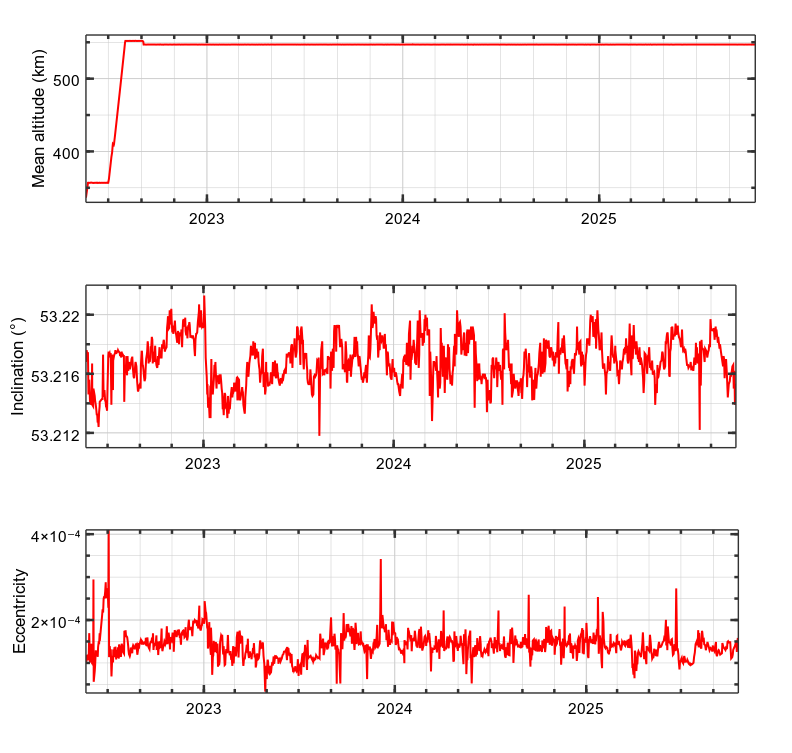
\includegraphics[width=\linewidth]{LaTeX/Figures/change_in_orbital_parameters.png}
%     \caption{Caption}
%     \label{fig:placeholder}
% \end{figure}

% \begin{figure}
%     \centering
%     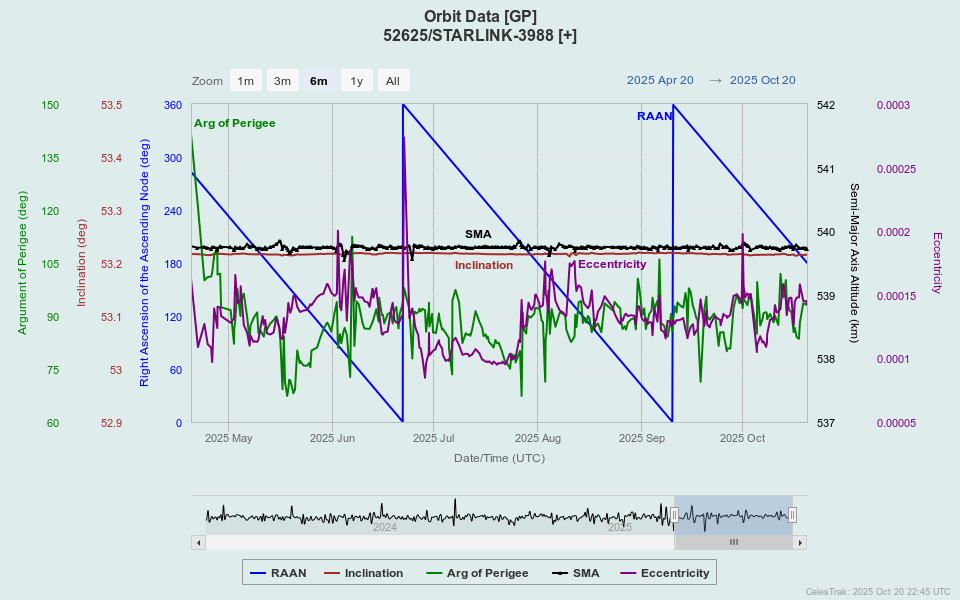
\includegraphics[width=\linewidth]{LaTeX/Figures/Orbit-Data-Starlink-3988.png}
%     \caption{Caption}
%     \label{fig:placeholder}
% \end{figure}

\section{Error Analysis}

\section{Conclusion}

\section{Visualisation}

\printbibliography

\newpage
\appendix
\section{Appendix} \label{Appendix}

Screenshots of the mobile apps used for the observations. The screenshots show the last observation taken on 10/20, and are labelled to distinguish them from other similar screenshots. Figure~\ref{fig:tracker_screenshot} shows the Satellite Tracker mobile app in use on a Samsung Galaxy S24 Ultra. Figure~\ref{fig:tracker_pro_screenshot} shows the Satellite Tracker Pro app in use on an iPhone 12.

\begin{figure}[h!]
    \centering

    \begin{subfigure}[b]{0.35\textwidth}
        \centering
        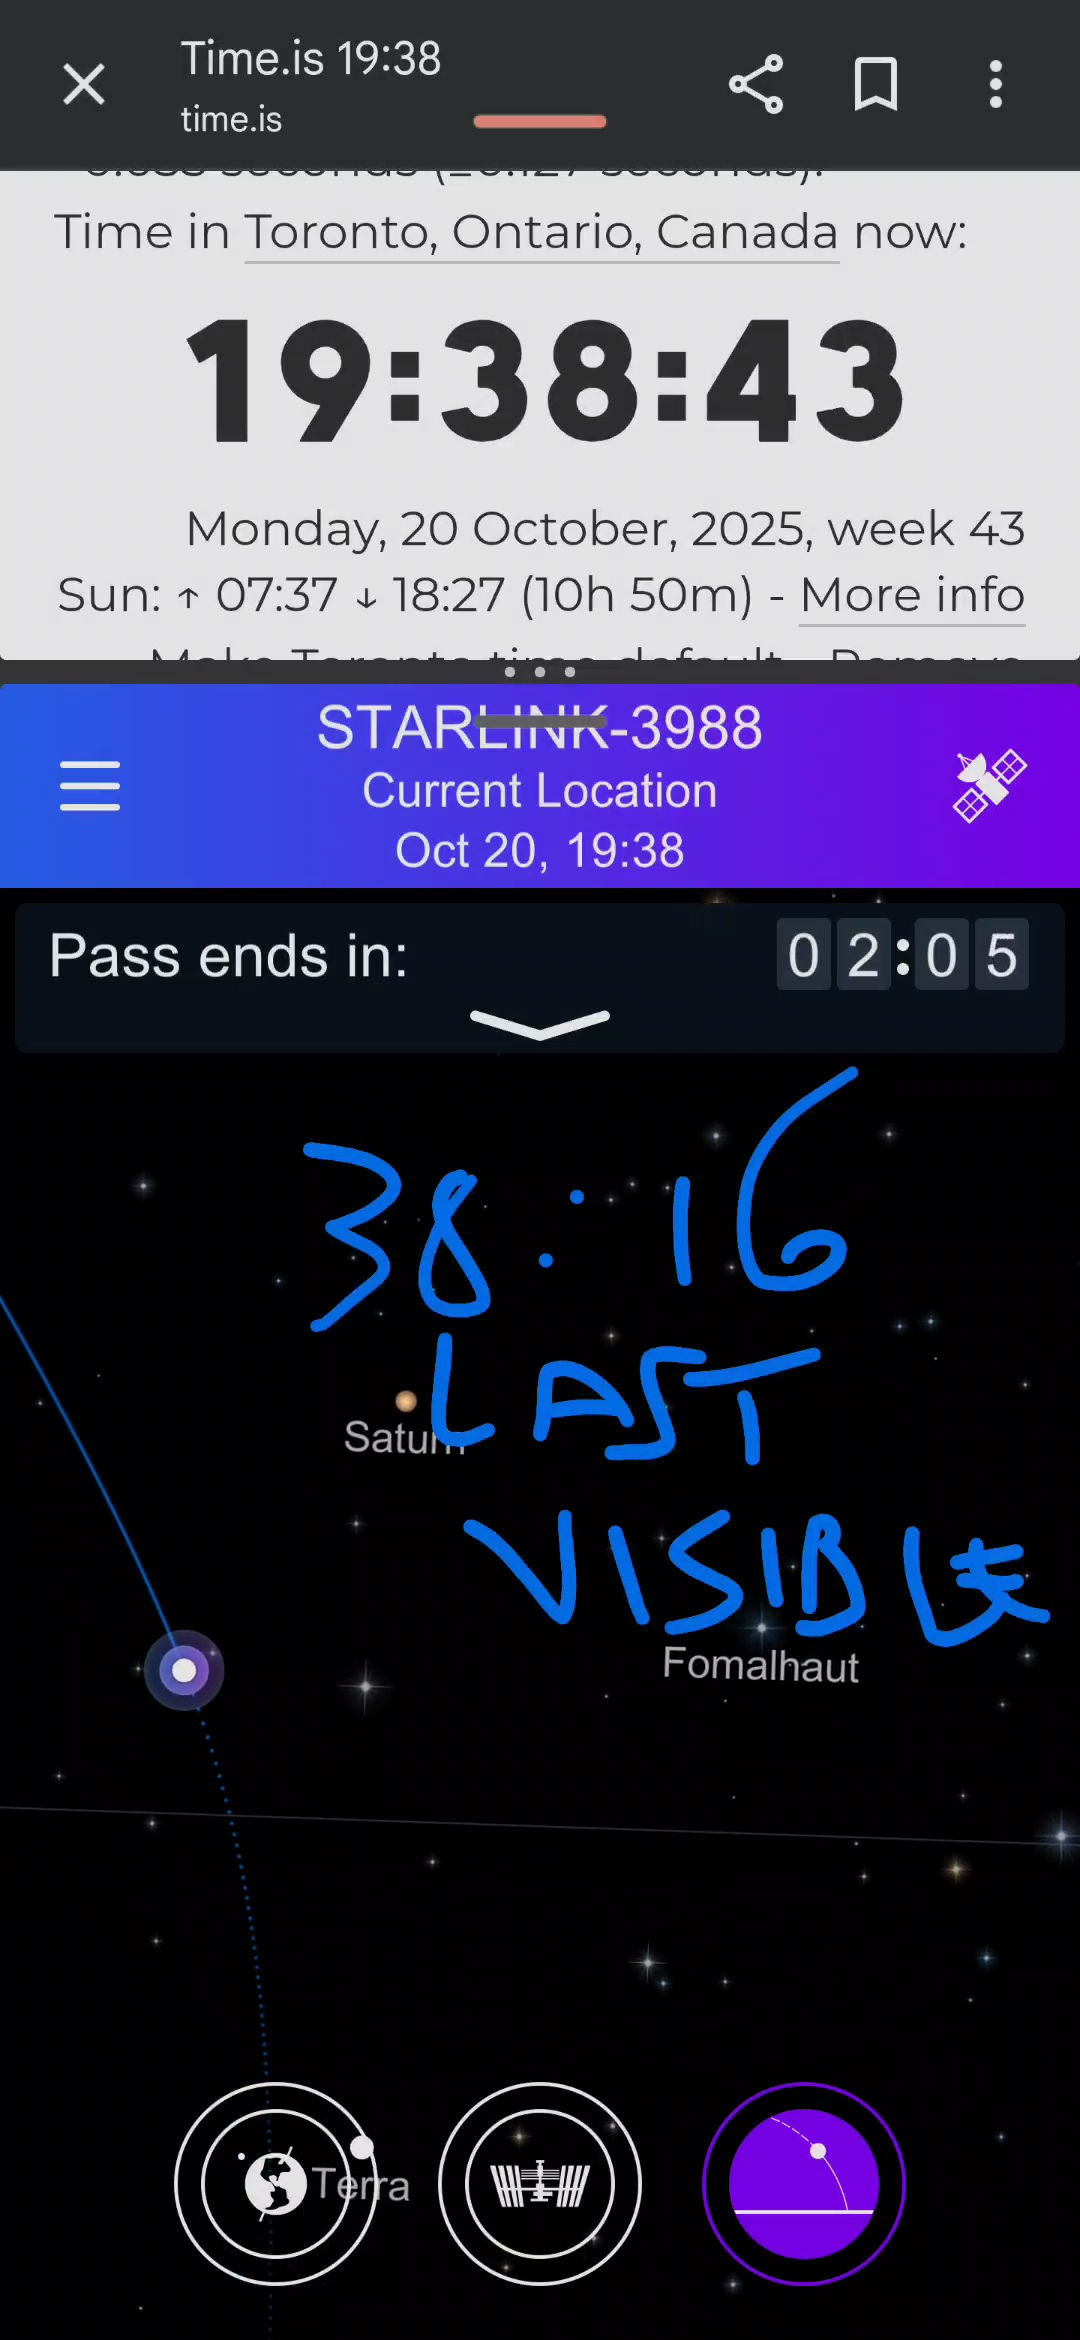
\includegraphics[width=\textwidth]{LaTeX/Figures/Satellite_Tracker_Screenshot.jpg}
        \caption{Satellite Tracker app}
        \label{fig:tracker_screenshot}
    \end{subfigure}
    \begin{subfigure}[b]{0.35\textwidth}
        \centering
        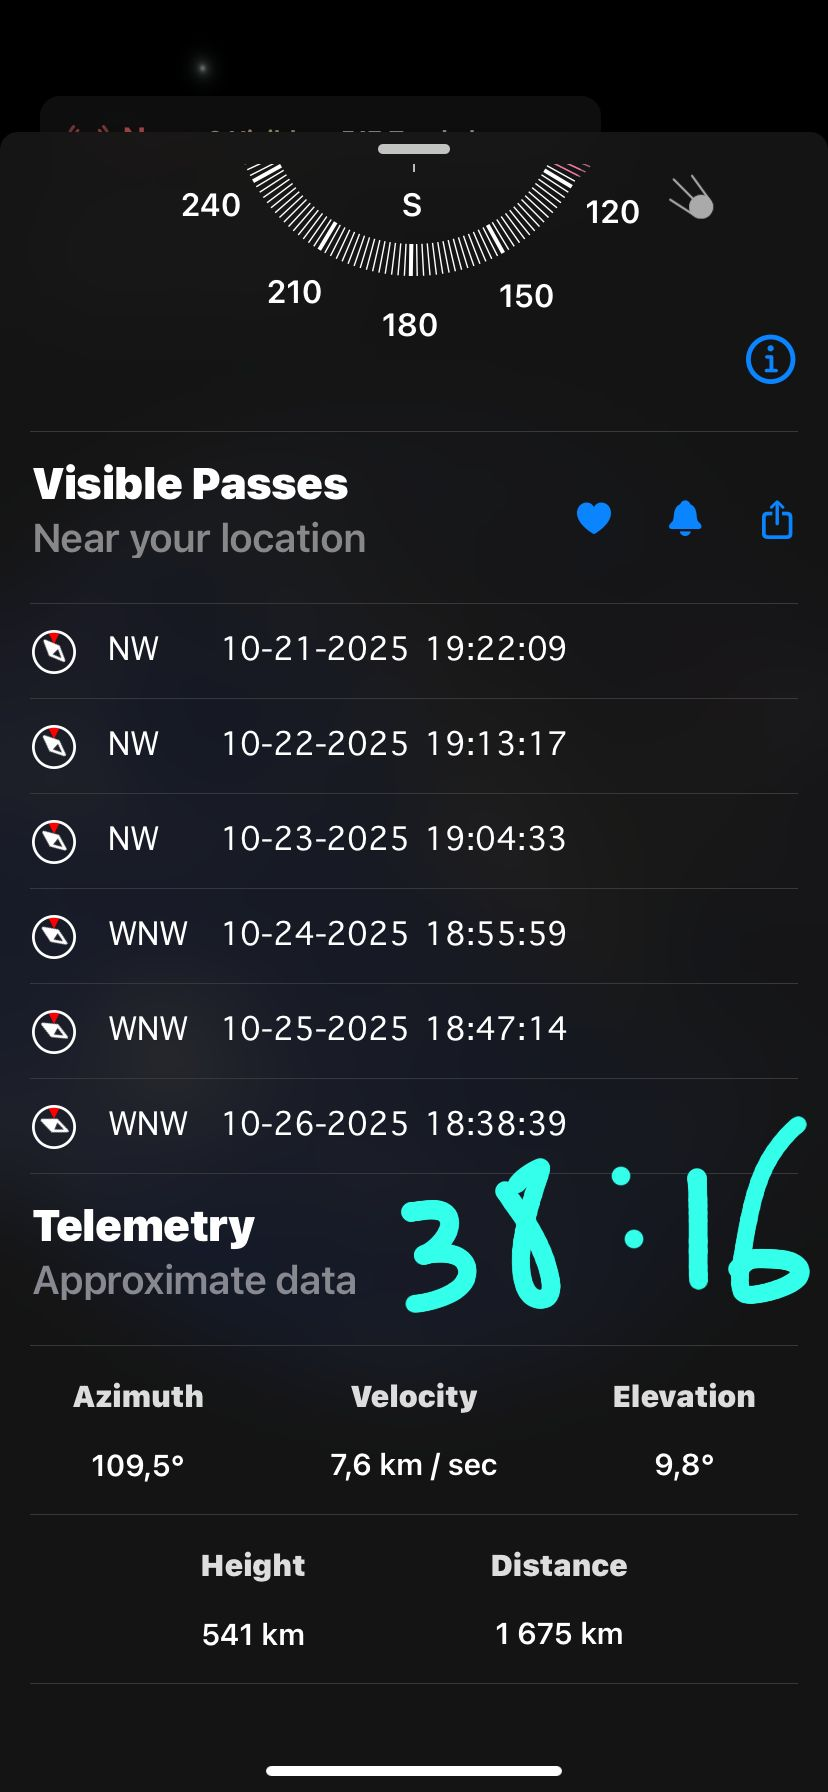
\includegraphics[width=\textwidth]{LaTeX/Figures/Satellite_Tracker_Pro_Screenshot.jpg}
        \caption{Satellite Tracker Pro app}
        \label{fig:tracker_pro_screenshot}
    \end{subfigure}
    
\end{figure}

Table~\ref{tab:method1_data_comparison} shows the data collected from the In The Sky website in preparation for the measurement later carried out with mobile apps for Method 1.

\begin{table}[H]
    \centering
    \caption{Comparison data from the In The Sky website}
    \label{tab:method1_data_comparison}
    \renewcommand{\arraystretch}{1.2}
    \begin{tabular}{|c|c|c|c|c|c|}
        \hline
        \textbf{Date} & \textbf{Time} & \textbf{Azimuth} & \textbf{Elevation} & \textbf{Right} & \textbf{Declination} \\ 
        \textbf{ } & \textbf{ } & \textbf{(°)} & \textbf{Angle (°)} & \textbf{Ascension (°)} & \textbf{(°)} \\ \hline
        \multicolumn{6}{|c|}{\textbf{Observation 1}} \\ \hline
        10/19 & 19:39:15 & 321.0 & 10.0 & 189.3 & 43.8 \\ \hline
        10/19 & 19:40:00 & 324.5 & 13.9 & 189.5 & 49.3 \\ \hline
        10/19 & 19:41:00 & 333.4 & 21.7 & 188.3 & 60.8 \\ \hline
        10/19 & 19:42:00 & 350.5 & 32.1 & 175.8 & 78.7 \\ \hline
        10/19 & 19:43:00 & 024.8 & 41.0 & 029.8 & 71.3 \\ \hline
        10/19 & 19:44:00 & 061.3 & 37.0 & 023.0 & 43.0 \\ \hline
        10/19 & 19:45:00 & 084.6 & 26.1 & 022.3 & 20.4 \\ \hline
        10/19 & 19:46:00 & 096.2 & 16.9 & 022.8 & 06.3 \\ \hline
        10/19 & 19:46:29 & 102.5 & 10.2 & 023.8 & -03.7 \\ \hline
    \end{tabular}
\end{table}

\newpage
Figure~\ref{fig:n2yo_screenshot} shows a screenshot of a frame from the screen recording of the N2YO website used for Method 4. The screen recording was carried out over several hours on a Windows 11 Razer Blade 14 using the Snipping Tool app.

\begin{figure}[h]
    \centering
    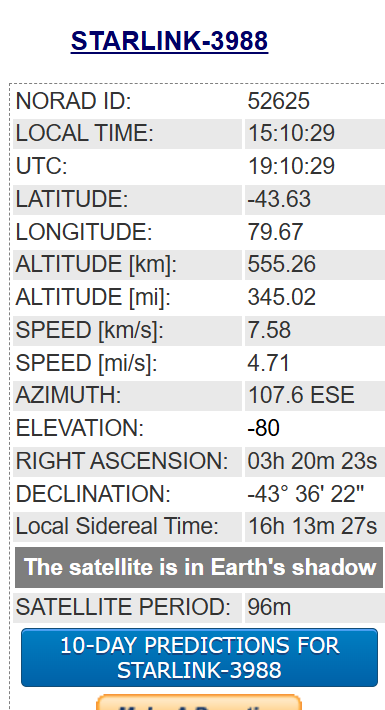
\includegraphics[width=0.5\linewidth]{LaTeX/Figures/N2YO .png}
    \caption{A frame from the screen recording of the N2YO website.}
    \label{fig:n2yo_screenshot}
\end{figure}

\newpage
\section*{Appendix B: Reading a Two-Line Element Set (TLE)}
\label{AppendixB}

Two-Line Element (TLE) sets provide the standard format used by NORAD and NASA to describe the orbital parameters of Earth-orbiting satellites. Each TLE consists of two lines of numerical data that together define the satellite's orbit at a given epoch. The TLE format is used by most satellite-tracking software and online resources, including N2YO~\cite{n2yo_starlink3988}, and is compatible with propagation models such as SGP4.

\noindent The following TLE corresponds to \textit{Starlink-3988}, obtained from N2YO on 21~October~2025:

\begin{verbatim}
1 52625U 22052AD  25294.95368970  .00001040  00000-0  83377-4 0  9997
2 52625  53.2146 171.9324 0001133  95.0058 265.1064 15.08848508190040
\end{verbatim}

\subsection*{Line 1: Identification and Timing Information}

\begin{itemize}
    \item Column 1: Line number (always 1 for the first line of the TLE).
    \item Columns 3 - 7: Satellite catalogue number. Here \texttt{52625} is the unique NORAD identification number assigned to \textit{Starlink-3988}.
    \item Column 8: Classification. The letter \texttt{U} indicates that the satellite is unclassified.
    \item Columns 10 - 17: International designator. The entry \texttt{22052AD} specifies the launch year (2022), the launch number (52), and the sequential piece identifier (AD).
    \item Columns 19 - 32: Epoch time. The value \texttt{25294.95368970} represents the year 2025 and the fractional day 294.95368970, corresponding to 21~October~2025 at 22:53:19~UTC (18:53:19 EDT). The epoch indicates the instant at which all the orbital parameters are valid.
    \item Columns 34--43: First time derivative of mean motion. The value \texttt{.00001040} represents the rate of change in the mean motion (revolutions per day) due to atmospheric drag.
    \item Columns 45 - 52: Second derivative of mean motion. The value \texttt{00000-0} is typically zero, as higher-order drag effects are negligible.
    \item Columns 54 - 61: BSTAR drag term. The value \texttt{83377-4} corresponds to a drag coefficient of \(8.3377\times10^{-4}\) (in reciprocal Earth radii). This parameter quantifies the effect of atmospheric drag on the satellite’s motion.
    \item Column 63: Ephemeris type. A value of \texttt{0} indicates use of the standard SGP4 orbital model.
    \item Columns 65 - 68: Element set number. The entry \texttt{999} identifies the current version of the orbital element set.
    \item Column 69: Checksum. The digit \texttt{7} ensures the integrity of the data line.
\end{itemize}

\subsection*{Line 2: Orbital Elements}

\begin{itemize}
    \item Column 1: Line number (always 2 for the second line of the TLE).
    \item Columns 3 - 7: Satellite number. The entry \texttt{52625} matches the value in Line~1.
    \item Columns 9 - 16: Inclination. The value \texttt{53.2146\si{\degree}} gives the angle between the orbital plane and the Earth's equatorial plane.
    \item Columns 18 - 25: Right Ascension of the Ascending Node (RAAN). The value \texttt{171.9324\si{\degree}} specifies the longitude where the satellite crosses the equator from south to north.
    \item Columns 27 - 33: Eccentricity. The digits \texttt{0001133} imply \(e = 0.0001133\). The decimal point is omitted in the TLE format but is understood to lie immediately before the first digit.
    \item Columns 35 - 42: Argument of Perigee. The value \texttt{95.0058\si{\degree}} is the angle, measured in the orbital plane, from the ascending node to the perigee.
    \item Columns 44 - 51: Mean Anomaly. The value \texttt{265.1064\si{\degree}} specifies the satellite’s position in its orbit at the epoch time.
    \item Columns 53 - 63: Mean Motion. The value \texttt{15.08848508} represents the number of orbital revolutions completed per sidereal day.
    \item Columns 64 - 68: Revolution number at epoch. The entry \texttt{19004} is the total number of orbits completed since launch.
    \item Column 69: Checksum. The digit \texttt{0} provides a line integrity check for the second line.
\end{itemize}

\subsection*{Derived Orbital Parameters}

From the mean motion \(n = 15.08848508~\si{rev/day}\), the orbital period is obtained as:
\[
\tau = \frac{1440}{n} = \SI{95.43}{\minute}.
\]
Using Kepler’s third law, the corresponding semi-major axis is determined as:
\[
a = \left(\frac{\mu}{(2\pi n / 86400)^{2}}\right)^{1/3} \approx \SI{6917}{\kilo\metre}.
\]
The eccentricity, inclination, and other parameters further allow for a calculation of the perigee and apogee altitudes:  the perigee and apogee distances (measured from the Earth's centre) are first obtained from the semi-major axis \(a\) and the orbital eccentricity \(e\) as:
\[
r_{p} = a(1 - e),
\qquad
r_{a} = a(1 + e).
\]
The corresponding altitudes above the Earth's surface are then:
\[
h_{p} = r_{p} - R_{E},
\qquad
h_{a} = r_{a} - R_{E},
\]
where \(R_{E}\) is the mean radius of the Earth. The mean orbital altitude \(h\) is the arithmetic mean of the perigee and apogee altitudes:
\[
h = \frac{h_{p} + h_{a}}{2}
    = \frac{(r_{p} - R_{E}) + (r_{a} - R_{E})}{2}
    = a - R_{E}.
\]
Hence, for nearly circular orbits (\(e \approx 0\)), the mean altitude simplifies to the difference between the semi-major axis and the Earth's mean radius. These TLEs were used to produce the orbital parameters summarised in Table~\ref{tab:starlink3988_orbit}.

\end{document}
